%\ihead{\headmark}
\chapter{Deep Learning}

Deep learning is a subfield of machine learning which is in fact, is a subfield of Artificial Intelligence (AI). Deep learning has emerged as one of the most exciting fields of computer science, and it keeps expanding its scope to other domains as well. It has been used in many technologies such as, in medical to identify the diseases, automatic game playing, self-driving cars, image recognition, and natural language processing. The reason why deep learning is successful in many different domains is its ability to understand multiple levels of representation of data. Its mean that, it not only has the ability to classify and predict but also has the ability to learn a different level of complexity. Before diving into deep learning, it is necessary to understand a broader ``machine learning''.

\section{Machine Learning}

Machine Learning is a data analysis method \cite{bishop2006pattern}. It gives the computer the ability to learn from data without being explicitly instructed. By using different machine learning algorithms, it helps to find hidden insights of data and allow us to build models to make predictions. It can be classified into 2 categories \cite{machinelearningmastery}.


\subsection{Supervised Learning}

In supervised learning, the labeled data is used to train the models. The labeled data represents that the input and output variables that are known in advance. Thus, a supervised machine learning algorithm is used to come up with a mapping function which maps the input variables to the output variables. Learning is supposed to be stopped when the level of performance reaches the desired result. Supervised learning is generally divided into regression and classification.
\begin{itemize}
	\item \textbf{Regression}: A problem in which the output variable is a category.
	\item \textbf{Classification}: A problem in which the output variable is the real value.
\end{itemize}

\subsection{Unsupervised Learning}

In unsupervised learning, only the input variables are known and no corresponding output variables are known. Thus, there are no labels given and it is expected from unsupervised machine learning algorithm to find the structure in the data, i.e. finding hidden patterns to learn more about data. It is different from supervised learning in that, the correct output values are not known. Unsupervised learning is generally divided into clustering and association.

\begin{itemize}
	\item \textbf{Clustering}: Group objects in such a way that the objects, which are similar to each other, placed in the same cluster.
	\item \textbf{Association}: Discover rules that define the large portions of the data such as people who buy product X may buy Y as well.
\end{itemize}

The objective of machine learning is to analyze the past and present data and predict or make a decision for the future data. In supervised learning, the basic workflow is to build a model, evaluate or tune a model and then deploy it in the production environment where it will make the predictions. The workflow can be seen in Figure \ref{fig:basic-ml-model}.


\begin{figure}[htpb]
	\centering
	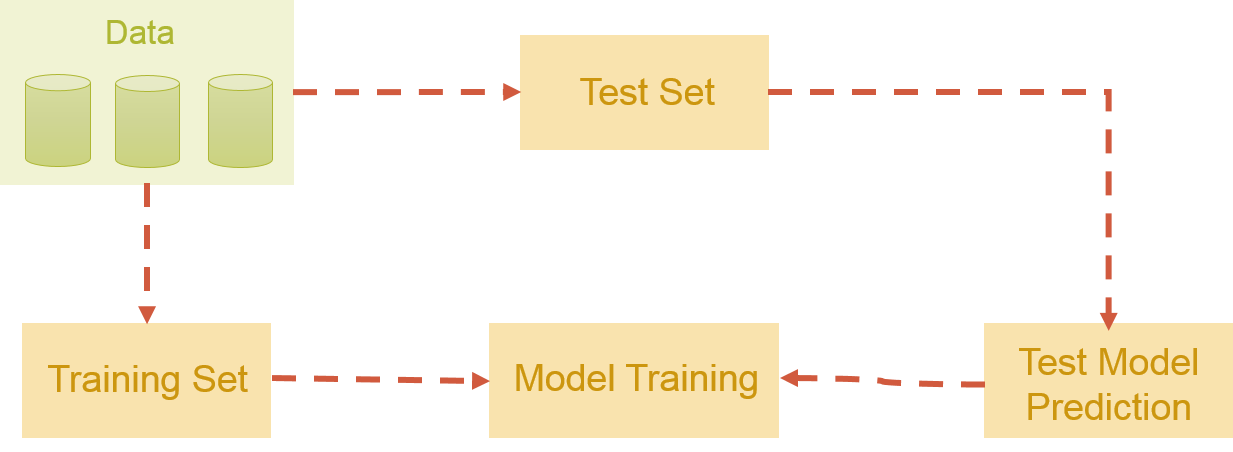
\includegraphics[width=12cm,height=10cm,keepaspectratio=true]{images/basic-ml-model.png}
	\caption{
		Basic supervised machine learning workflow.
	}
	\label{fig:basic-ml-model}
\end{figure}


Machine learning is generally powered by a huge amount of data which is generally referred as Big Data. It is generally defined as a too big or complex data which cannot be processed on a single machine. As the data is growing day by day, the new tools are also required to process that big data on multiple machines and extract the useful insights from the data.


One of the problems with the traditional machine learning model is the feature extraction challenge. The model designer or the programmer need to specifically tell the model which features it should consider while making a decision. The model heavily relies on the programmer's understanding of data and this was a huge burden on the programmers. For problems like object recognition and language translation, it was considered as a huge problem.

Deep learning comes into play to solve the problem of feature extraction. They have the capability to focus only on the right features by themselves by understanding as much data as possible, requiring very little input from the programmer. This feature of deep learning models makes it very powerful tool for the current machine learning era.


\section{Artificial Neural Networks}
Artificial neural networks (ANNs) are generally inspired by the biological neural networks that mimic brain functionality \cite{wiki:ann}. These systems generally learned by considering examples instead of specifically define rules for certain situations or cases. An ANN is a network of nodes called artificial neurons which are connected to other neurons using a link called \textit{synapse}. Each neuron gets the input, process the input and pass the output to the next neuron.
In the most basic state, an ANN consists of 3 layers:

\begin{enumerate}
	\item Input Layer
	\item Hidden Layer
	\item Output Layer
\end{enumerate}

\begin{figure}[htpb]
	\centering
	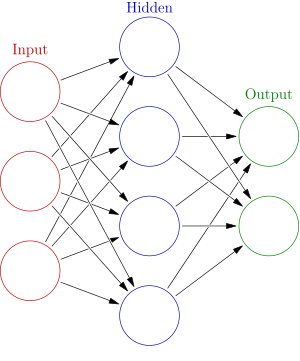
\includegraphics[width=6cm,height=10cm,keepaspectratio=true]{images/neural-net}
	\caption{
		An artificial neural network with its 3 basic layers \cite{wiki:ann}.
	}
	\label{fig:wiki:ann}
\end{figure}


\subsection{Artificial Neuron}
An artificial neuron is the most basic unit of ANN. It takes inputs and produces an output. Generally, the inputs are multiplied by some weights to specify which inputs are more important. The higher the value of weight is, the more important it is. The inputs are shown as a, b, and c, and weights as $w_1$, $w_2$ and $w_3$ in Figure \ref{fig:single-neuron}. After then the products are summed together and passed to the activation function. So, if the summed value is greater than the threshold value of the activation function, the output is produced or in other terms, the neuron fired else no output is produced and neuron does not fire.

\begin{figure}[htpb]
	\centering
	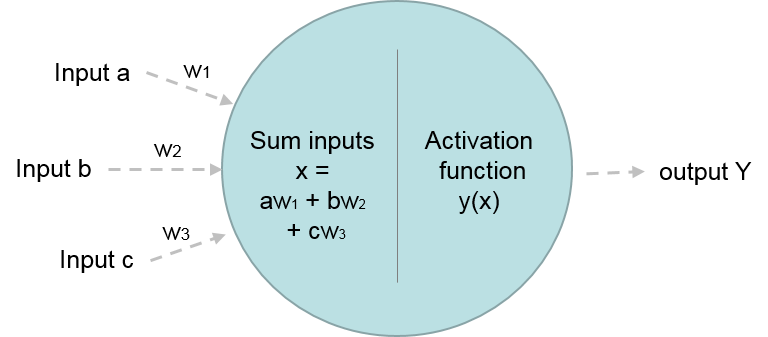
\includegraphics[width=10cm,height=10cm,keepaspectratio=true]{images/single-neuron}
	\caption{
		A single artificial neuron.
	}
	\label{fig:single-neuron}
\end{figure}

Artificial neurons adjust the weights as the learning proceeds and the process of finding weights is known as learning. ANN considers many different examples and finds the best possible combination of weights to provide the most accurate results. There are many other parameters involved as well to find a good combination of weights.

\subsection{Activation Function}

A function that takes an input and produces output based on threshold value is known as activation function \cite{ujjwalkarn}. There are many activation functions available. Few of them are:

\subsubsection{Sigmoid}
It takes a real value input and scales it to the range of 0 to 1. It is also known as the logistic function. It is represented as:

\begin{equation} 
y = \frac{1}{1 + e^{-x}}
\end{equation}

Another variation of the sigmoid function is softmax function which is used for multiclass classification.

\subsubsection{Tanh}
It takes a real value input and scales it to the range of -1 to 1. It is also a sigmoidal function as it also takes s-shaped.


\subsubsection{ReLU}
It stands for Rectified Linear Unit. It is the most used activation function with convolutional neural networks\cite{ujjwalkarn}. It takes the real value input and all negative values are mapped to zero. It is represented as:

\begin{center}
	$f(x) = max(0, x)$
\end{center}

\begin{figure}[htpb]
	\centering
	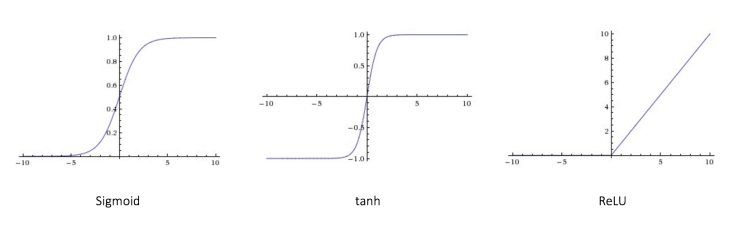
\includegraphics[width=15cm,height=10cm,keepaspectratio=true]{images/act-funcs}
	\caption{
		Activation functions \cite{ujjwalkarn}.
	}
	\label{fig:funcs}
\end{figure}

The graph of all the activation functions defined above can be seen in Figure \ref{fig:funcs}.

\subsection{Convolutional Neural Network}
Convolutional neural network (CNN) is a class of deep neural network which uses multilayer perceptrons. It consists of an input layer, an output layer, and multiple hidden layers. The hidden layers can be convolutional, pooling or fully connected layer. An example of CNN is shown is Figure \ref{fig:cnn_1d}. 

\begin{figure}[htpb]
	\centering
	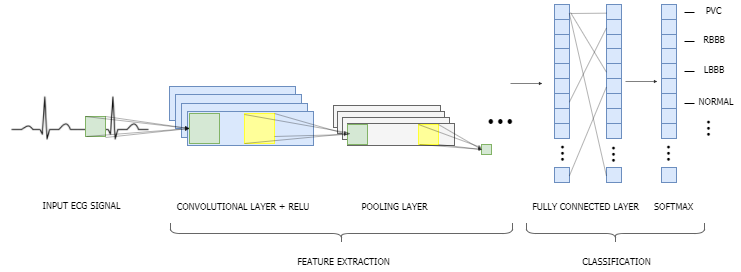
\includegraphics[width=15cm,height=15cm,keepaspectratio=true]{images/cnn_1d}
	\caption{
		Convolutional neural network example.
	}
	\label{fig:cnn_1d}
\end{figure}

\subsubsection{Convolutional Layer}
In CNN, the first layer is always the convolutional layer. This layer applies a convolutional operation to the input and passes the output to the next layer. A filter (or sometimes referred as a kernel) is used which slides over all the area of the input and extract the features from it. The region where the filter is being applied at any instant of time is called as a receptive field. As the filter slides or convolves over the input signal, it multiples the filter with the original signal values (which can also be referred as element-wise multiplication) which results in a single value. The important point to note here is that this single result is just from a single receptive field. Therefore, the same operation will be carried out on other receptive fields by sliding the filter over the different areas of the input signal. The filter can slide for any unit and this sliding unit is known as stride. Every unique area of the input signal will produce an output and the combined output together is called as feature map or an activation map.  If we assume that, the input size is 32x32, the filter size is 5x5 and the stride is 1 unit, then the size of the activation map will be 28x28. In a 2D array, the filter can be moved in both directions.

\subsubsection{Pooling Layer}
Pooling layer is used to downsampled the convolutional layer output. There are several pooling options, for example, average pooling and L2-norm pooling, but max pooling is the most popular. This layer basically takes a filter of size 2x2 with the same stride size. It then applies the filter to the part of input and output the maximum number in that region. The same process is applied to the different sub-region by sliding the filter all over the input. By convolving the filter around the input, it drastically reduces the spatial size of the input. The example of how pooling layer work is shown in Figure \ref{fig:maxpool}.

\begin{figure}[htpb]
	\centering
	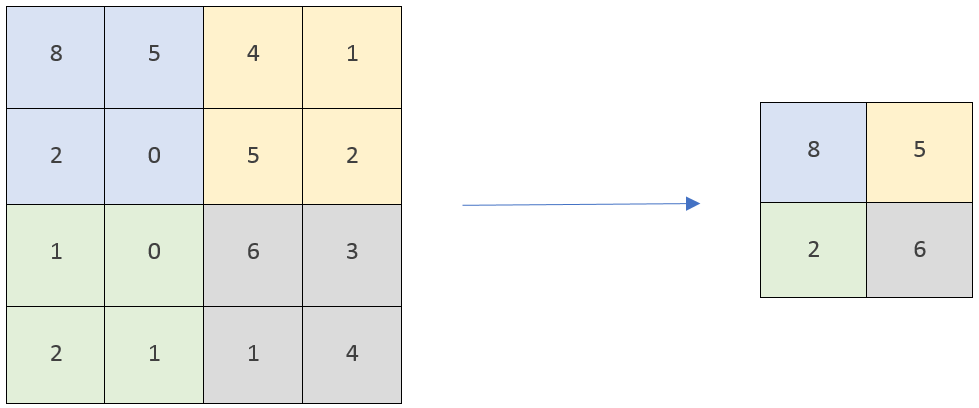
\includegraphics[width=12cm,height=10cm,keepaspectratio=true]{images/maxpool}
	\caption{
		Max pooling layer example.
	}
	\label{fig:maxpool}
\end{figure}

\subsubsection{Fully Connected Layer}
In a fully connected layer, the neurons of one layer are connected to all the neurons of the second layer, as shown in Figure \ref{fig:cnn_1d}. This layer can be seen in the regular neural network as well. The softmax function is applied to the output of the second layer to produce the probabilities for the classification of the input. 

\subsection{Keras}

Keras is an open source artificial neural network library written in python. It is very powerful and easy to use library to develop neural networks. It has a capability to run on top of TensorFlow, Microsoft Cognitive Toolkit (CNTK), or Theano, can run on both CPU and GPU. Before Keras, it was really time-consuming to develop a network on TensorFlow or Theano and the aim to develop Keras is to make it easy and fast to develop neural networks. Keras supports both convolutional neural networks and recurrent neural network, as well as a combination of both.

The model starts by defining the model as sequential using a \textit{Sequential()}, which is a linear stack of layers. Then the layers are added into the model using \textit{add()} method. Keras supports almost all kinds of layers. The input dimensions are needed to specify when the layers are added to the model. Once the layers are added, the model is compiled by using the \textit{compile()} method, which additionally needs 3 arguments.

\begin{itemize}
	\item Optimizer: It is used to optimize the neural network. Examples of optimizer are RSE, Adagrad and Adam.
	\item Loss Function: This is the value that model tries to minimize to calculate the error. For example, categorical cross-entropy and MSE.
	\item Metrics: It can be any existing metric or a custom defined metric function. But for classification problems metrics=['accuracy'] is recommended.
\end{itemize}

The model is trained by using the \textit{fit()} method. This method lets the model iterate over the data and finds the most optimal neural network for the given data.

Keras has been used for training the CNN to identify cardiac arrhythmias.


\begin{figure}[htpb]
	\centering
	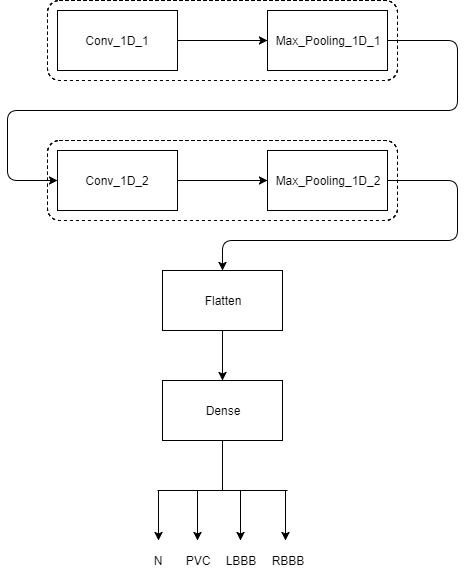
\includegraphics[width=20cm,height=15cm,keepaspectratio=true]{images/cnn_model}
	\caption{
		A 6-layer Convolutional Neural Network model for the identification of cardiac arrhythmia.
	}
	\label{fig:cnn_model}
\end{figure}


\subsection{Convolutional Neural Network for the Identification of Cardiac Arrhythmia}
A 6-layer Convolutional Neural Network (CNN) has been trained for the identification of an arrhythmia in an ECG signal. The trained model can detect 3 different kinds of arrhythmia namely:

\begin{enumerate}
	\item Normal
	\item Left bundle branch block (LBBB)
	\item Right bundle branch block (RBBB)
	\item Premature ventricular contraction (PVC)
\end{enumerate}

The CNN layers are shown in Figure \ref{fig:cnn_model}.

\begin{figure}[htpb]
	\centering
	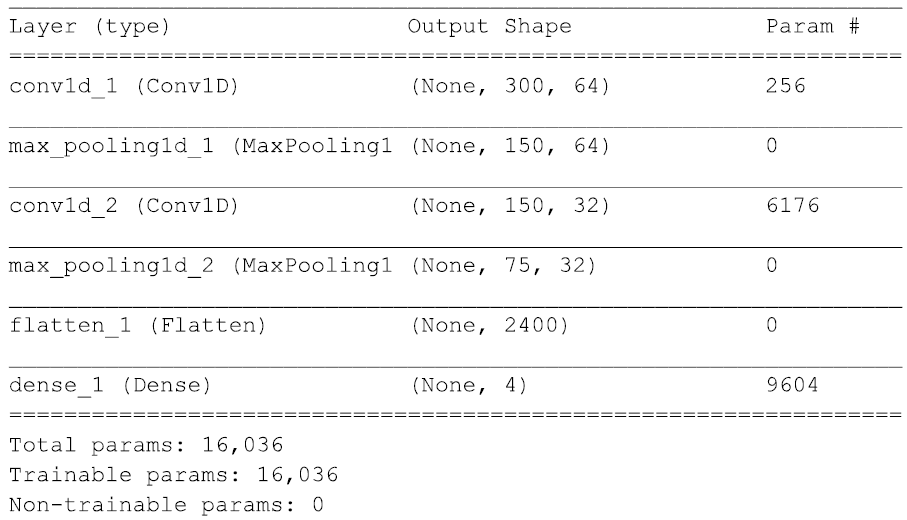
\includegraphics[width=12cm,height=10cm,keepaspectratio=true]{images/model_def_var}
	\caption{
		Layers used in the model and number of parameters to be optimized.
	}
	\label{fig:model_def_var_opt}
\end{figure}



\begin{figure}%
	\centering
	
	\subfigure[][]{%
		\label{fig:ex3-c}%
		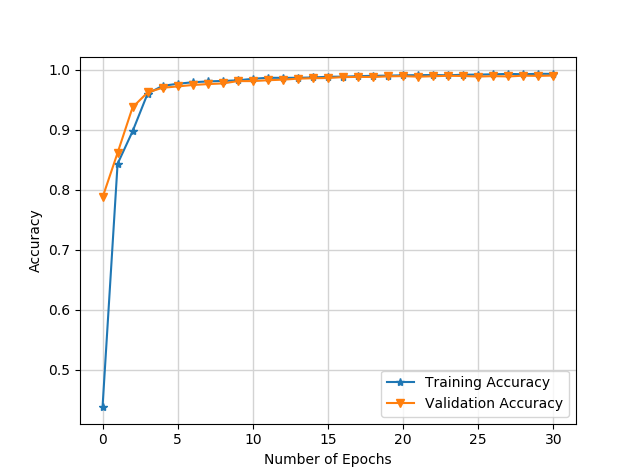
\includegraphics[height=4in]{images/acc}}%
	\hspace{8pt}%
	\subfigure[][]{%
		\label{fig:ex3-d}%
		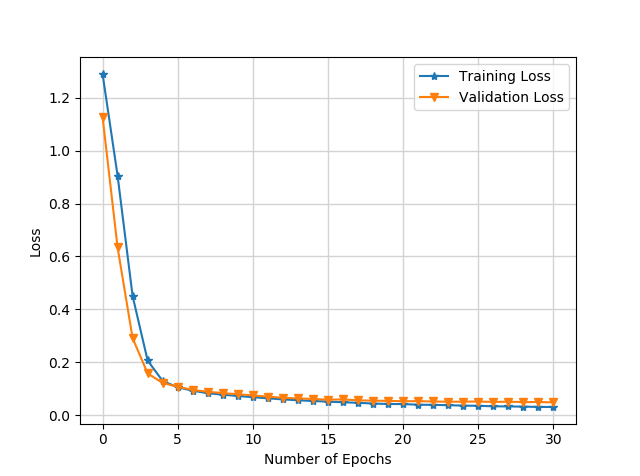
\includegraphics[height=4in]{images/val}}%
	\caption[A set of four subfigures.]{
		\subref{fig:ex3-c} Training and validation accuracy results; and,
		\subref{fig:ex3-d} training and validation loss of CNN model for 30 iterations.}%
	\label{fig:acc_val}%
\end{figure}




\subsubsection{Layers Explanation}
The 1st convolutional layer (Conv\_1D\_1) consists of 64 filters, whereas, the 2nd convolutional layer (Conv\_1D\_2) consists of 32 filters with a kernel of size 3. The model need to optimize total of 16,036 params to find an optimal CNN, as shown in Figure \ref{fig:model_def_var_opt}. For both convolutional layers, Relu has been used as an activation function each followed by a max-pooling layer. The batch size of 1,000 was used for the training, along with the Adam algorithm to optimize the CNN. Since the model is trained for performing the classification of an ECG signal, therefore, categorical cross-entropy loss function is used for calculating the loss of training and validation. After performing the convolutions, the flattening and dense layer has been used, followed by a softmax activation function to produce the final probabilities with 4 different classes.


The model is trained and tested for the several numbers of iterations ranging from 10 to 100. The best model was found after 20 iterations. After that, the model remained stable with the slight improvement in the training as well as in the validation accuracy. The training and validation accuracy can be seen in Figure \ref{fig:acc_val}.



\subsubsection{Results}
The CNN model has achieved an accuracy of 99.2\% on MIT-BIH dataset. Total 16,415 ECG signals were extracted from the MIT-BIH dataset, out of which 10,998 (67\% of the total signals) were used for the training, and the remaining 5,417 (33\% of the total signals) were used for the testing of the model. The types count for training and testing data can be seen in Tables \ref{tab:train_count} and \ref{tab:test_count} respectively. 

\renewcommand{\arraystretch}{2}
\begin{table}
	\caption{Training data.} \label{tab:train_count}
	
	\begin{center}
		\begin{tabular}{ | l | r | }
			\hline
			\textbf{Type} & \textbf{Count} \\ \hline
			Normal & 3,352 \\ \hline
			LBBB  & 2,641  \\ \hline
			RBBB  & 2,498  \\ \hline
			PVC  & 2,507  \\ \hline
			\textbf{Total}  & \textbf{10,998}  \\ \hline
		\end{tabular}
	\end{center}
	
\end{table}


\renewcommand{\arraystretch}{2}
\begin{table}
	\caption{Test data.} \label{tab:test_count}
	
	\begin{center}
		\begin{tabular}{ | l | r | }
			\hline
			\textbf{Type} & \textbf{Count} \\ \hline
			Normal & 1,648 \\ \hline
			LBBB  & 1,308  \\ \hline
			RBBB  & 1,285  \\ \hline
			PVC  & 1,176  \\ \hline
			\textbf{Total}  & \textbf{5,417}  \\ \hline
		\end{tabular}
	\end{center}
	
\end{table}

During the testing of the model, 42 ECG signals were classified wrong out of 5,417 ECG signals. The false predicted results can be seen in Table \ref{tab:false_pred_count}. In the table, $a \rightarrow b$ represents that $a$ was classified as $b$.


\renewcommand{\arraystretch}{2}
\begin{table}
	\caption{False prediction counts.} \label{tab:false_pred_count}
	
	\begin{center}
		\begin{tabular}{ | l | r | }
			\hline
			\textbf{False Prediction} & \textbf{Count} \\ \hline
			0 $\rightarrow$ 1  & 1   \\ \hline
			0 $\rightarrow$ 2  & 1  \\ \hline
			0 $\rightarrow$ 3  & 3  \\ \hline
			1 $\rightarrow$ 3  & 6  \\ \hline
			2 $\rightarrow$ 0  & 5  \\ \hline
			2 $\rightarrow$ 3  & 3  \\ \hline
			3 $\rightarrow$ 0  & 9  \\ \hline
			3 $\rightarrow$ 1  & 12 \\ \hline
			3 $\rightarrow$ 2  & 2  \\ \hline
			\textbf{Total}   & \textbf{42}  \\ \hline
		\end{tabular}
	\end{center}
	
\end{table}